\begin{figure*}[h]
    \centering
    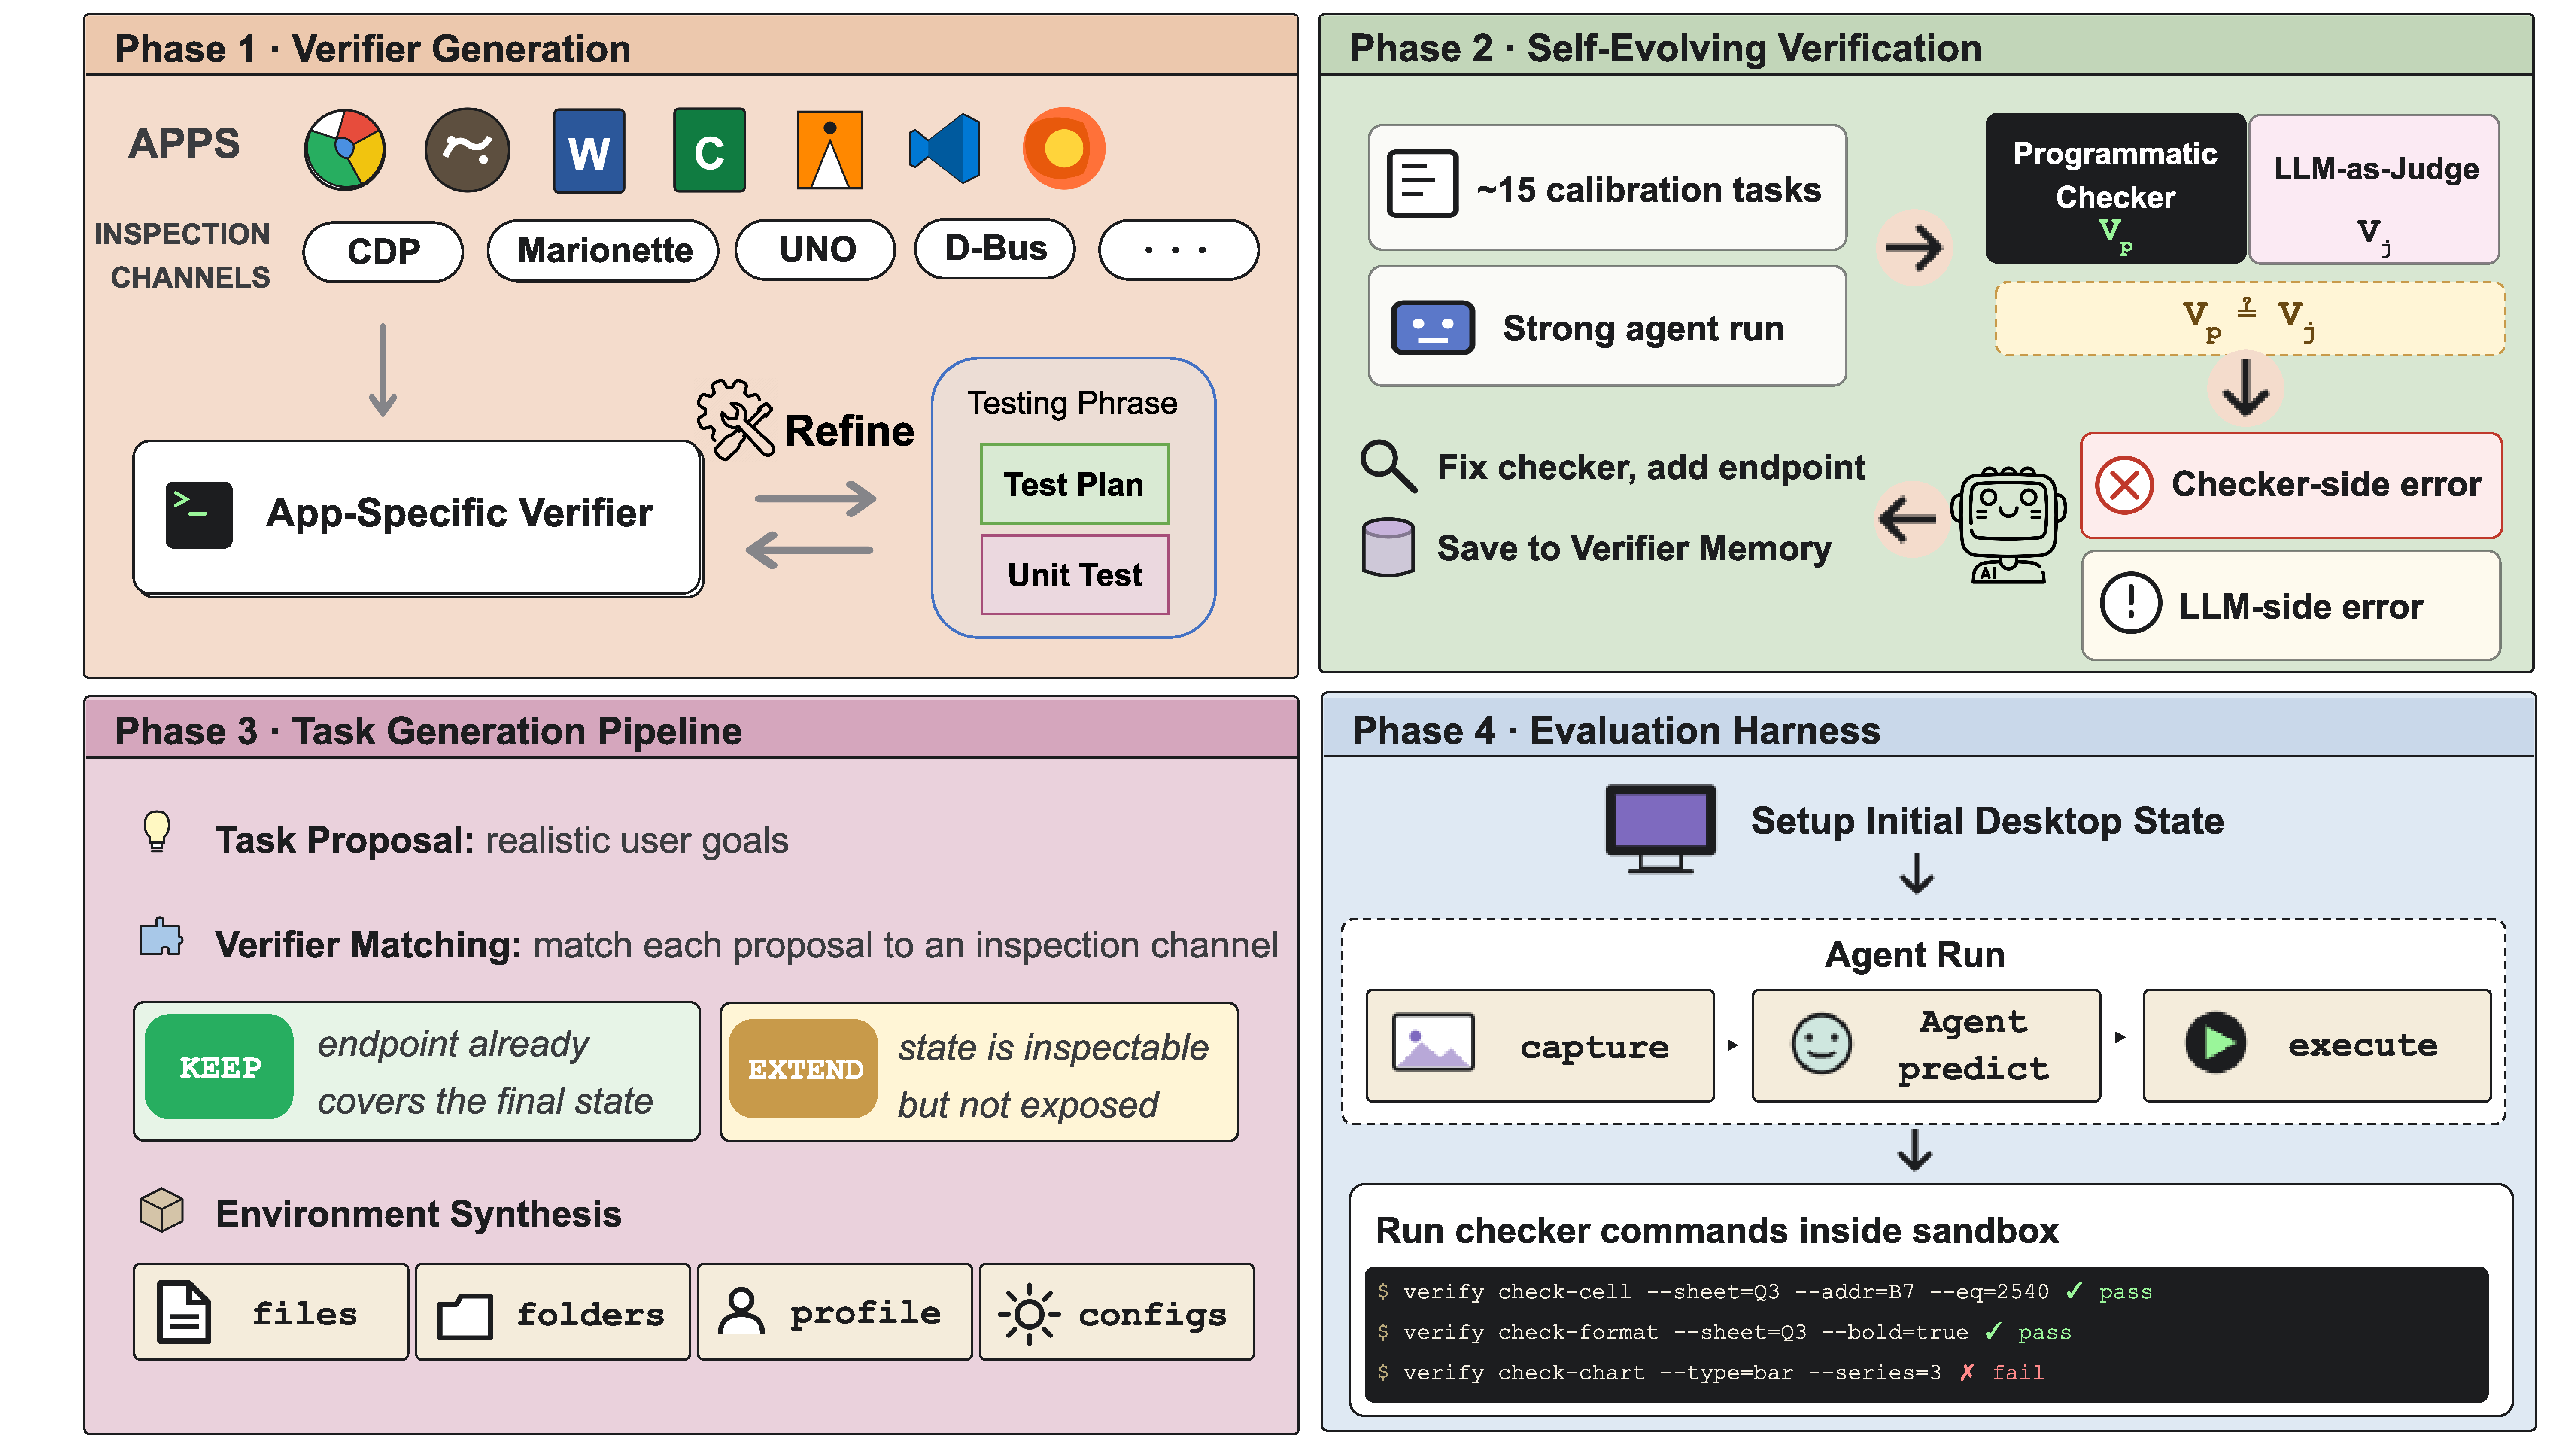
\includegraphics[width=0.95\textwidth]{image/main_figure.pdf}
    \caption{ Overview of the OpenComputer verifiable software-world synthesis pipeline. Phase 1 generates app-specific verifier endpoints over the most reliable inspection channels and validates it with unit and integration tests for structured, machine-checkable state. Phase 2 closes a self-evolving loop: calibration tasks drive a strong agent run, an LLM evaluator and the programmatic verifier produce verdicts that disagreement analysis attributes, and verifier memory + checker/endpoint/doc fixes refine the verifier with execution-grounded feedback. Phase 3 proposes user goals, filters by complexity and data generatability, matches against the verifier, synthesizes the environment, and emits a final task instance. Phase 4 runs the agent and computes the reward.}
    \label{fig:opencomputer-pipeline}
\end{figure*}


\section{Introduction}
Computer-use agents offer a promising path toward general-purpose AI systems that operate the same software interfaces humans use every day~\citep{agasheagent,nguyen2025gui,agashe2025agent,song2025coact}, but scaling their training and evaluation is limited by the cost of constructing realistic, reproducible desktop environments and tasks~\citep{xu2024agenttrek, he2024pc}. 

Constructing a realistic desktop task involves far more than writing a natural-language instruction. A human developer must first design a plausible user goal, then manually prepare the underlying environment state (\eg creating or editing files, configuring folders, populating spreadsheets or documents, setting browser history or bookmarks, preparing emails or calendars), and ensures that the software state is both coherent and reproducible~\cite{xie2024osworld,bonatti2024windows}. These steps are tedious, application-specific, and difficult to standardize, making large-scale task creation slow and expensive.

Beyond environment construction, computer-use tasks also require trustworthy verification of the resulting software state. In desktop settings, success is often reflected not only in visible screenshots, but also in application state, file contents, metadata, or persistent side effects~\cite{xie2024osworld,bonatti2024windows}. This makes evaluation difficult to scale: each task often requires custom inspection logic that can determine whether the intended state has actually been achieved. A natural fallback is to use an LLM-as-a-judge~\cite{liu2023g,kim2024prometheus}, but this introduces substantial limitations. LLM judgments can be sensitive to prompt wording, incomplete observations, and model-specific biases, and are often difficult to audit or reproduce across runs~\citep{wang2024large,li2025generation,thakur2025judging,zheng2023judging}. More importantly, an LLM judge may reward outcomes that appear plausible from screenshots while missing errors in the underlying software state~\citep{sumyk2026cuaaudit,cui2026agentic}. Thus, scalable synthesis for computer-use agents must be coupled with reliable inspection rather than weak proxy evaluation.

To address the dual bottlenecks of scalable environment construction and trustworthy state verification, we present \textbf{\ours}, a verifier-grounded framework for synthesizing verifiable software worlds for computer-use agents. Rather than treating verification as a downstream evaluation detail, \ours makes verification the organizing principle of environment and task construction.
It consists of four tightly coupled components as illustrated in Figure~\ref{fig:opencomputer-pipeline}. First, it builds app-specific state verifiers that undergo a strict debug-fix-retry testing loop to reliably inspect software state through stable interfaces, defining exactly which task outcomes can be checked programmatically. Second, it further improves these verifiers through an execution-grounded self-evolution loop: calibration tasks are executed in sandboxed desktops, programmatic verifier outputs are compared against criterion-level LLM judgments, and verifier-side failures are used to refine checker logic, endpoints, or documentation. Third, on top of this verifier stack, \ours synthesizes realistic user tasks through a structured pipeline that filters for difficulty, data generatability, and state inspectability. Finally, \ours provides an evaluation harness that runs agents in fresh desktop sandboxes, records full screenshot-action trajectories, and scores each run by executing verifier commands over the resulting software state.

Empirically, \ours shows that current computer-use agents still struggle to reliably complete realistic desktop tasks end to end. GPT-5.4 achieves the strongest overall performance, with a full task success rate of 68.3\%, while Claude-Sonnet-4.6 and Kimi-K2.6 reach 64.4\% and 58.8\%, respectively. Open-source agents lag substantially behind, with especially large drops relative to their reported performance on existing desktop benchmarks such as OSWorld~\cite{xie2024osworld}. Our analysis further highlights the importance of verifier-grounded benchmark construction. Hard-coded verifiers align more closely with human adjudication than an agentic LLM judge, particularly when success depends on fine-grained application state that cannot be reliably inferred from screenshots alone.

We summarize our contributions as follows:
\begin{enumerate}[leftmargin=*, itemsep=2pt]
    \item We introduce \ours, a verifier-grounded framework for synthesizing realistic software worlds for computer-use agents, where the task descriptions, environments, and verifiers for evaluation are all automatically generated without relying on manual construction.
    
    \item We empirically validate the reliability of this construction pipeline, showing that verifier-grounded evaluation aligns more closely with human adjudication than LLM-as-judge evaluation, and that the self-evolving verification layer can identify and repair verifier-side failures.

    \item We instantiate a large-scale benchmark spanning \napp desktop applications and \nexample finalized tasks, and evaluate frontier and open-source computer-use agents to show that realistic, verifier-grounded desktop workflows remain challenging for current systems.
\end{enumerate}
